\documentclass[a4paper,11pt]{book}
%\documentclass[a4paper,twoside,11pt,titlepage]{book}
\usepackage{listings}
\usepackage[utf8]{inputenc}
\usepackage{marvosym}
\usepackage[spanish]{babel}

\usepackage[acronym, numberedsection=autolabel, entrycounter]{glossaries} %
\usepackage{amsmath} 
\usepackage{nameref}
%\usepackage{titlesec}
%\usepackage{pailatino}
\usepackage{appendix}
\decimalpoint
\usepackage{dcolumn}
\newcolumntype{.}{D{.}{\esperiod}{-1}}
\makeatletter
\addto\shorthandsspanish{\let\esperiod\es@period@code}
\makeatother


%\usepackage[chapter]{algorithm}
\usepackage{algorithm}
\usepackage[noend]{algpseudocode}

\RequirePackage{verbatim}
%\RequirePackage[Glenn]{fncychap}
\usepackage{fancyhdr}
\usepackage{graphicx}
\usepackage{afterpage}
\usepackage{xspace}
\usepackage{longtable}

\usepackage[pdfborder={000}]{hyperref} %referencia

% ********************************************************************
% Re-usable information
% ********************************************************************
\newcommand{\myTitle}{Desarrollo de un prototipo de motor de búsqueda que incorpore técnicas bibliométricas para mejorar la recuperación\xspace}
\newcommand{\myDegree}{Master Universitario en Ingeniería Informática\xspace}
\newcommand{\myName}{Aythami Estévez Olivas\xspace}
\newcommand{\myProf}{Juan Manuel Fernández Luna\xspace}
\newcommand{\myOtherProf}{Nombre Apllido1 Apellido2 (tutor2)\xspace}
%\newcommand{\mySupervisor}{Put name here\xspace}
\newcommand{\myFaculty}{Escuela Técnica Superior de Ingenierías Informática y de
Telecomunicación\xspace}
\newcommand{\myFacultyShort}{E.T.S.I.I.T.\xspace}
\newcommand{\myDepartment}{Departamento de Ciencias de la Computación e Inteligencia Artificial\xspace}
\newcommand{\myUni}{\protect{Universidad de Granada}\xspace}
\newcommand{\myLocation}{Granada\xspace}
\newcommand{\myTime}{\today\xspace}
\newcommand{\myVersion}{Version 0.1\xspace}
\DeclareUnicodeCharacter{20AC}{\EUR{}}

\hypersetup{
urlcolor=blue,
pdfauthor = {\myName (aythae (at) correo (punto) ugr (punto) es)},
pdftitle = {\myTitle},
pdfsubject = {},
pdfkeywords = {palabra_clave1, palabra_clave2, palabra_clave3, ...},
pdfcreator = {LaTeX con el paquete pdflatex},
pdfproducer = {pdflatex}
}

%\hyphenation{}


%\usepackage{doxygen/doxygen}
%\usepackage{pdfpages}
\usepackage{url}
\usepackage{colortbl,longtable}
\usepackage[stable]{footmisc}
%\usepackage{index}

%\makeindex
%\usepackage[style=long, cols=2,border=plain,toc=true,number=none]{glossary}
% \makeglossary

% Definición de comandos que me son tiles:
%\renewcommand{\indexname}{Índice alfabético}
%\renewcommand{\glossaryname}{Glosario}
\renewcommand{\appendixname}{Anexos}
\renewcommand{\appendixtocname}{Anexos}
\renewcommand{\appendixpagename}{Anexos}
\pagestyle{fancy}
\fancyhf{}
\fancyhead[LO]{\leftmark}
\fancyhead[RE]{\rightmark}
\fancyhead[RO,LE]{\textbf{\thepage}}
\renewcommand{\chaptermark}[1]{\markboth{\textbf{#1}}{}}
\renewcommand{\sectionmark}[1]{\markright{\textbf{\thesection. #1}}}

\setlength{\headheight}{1.5\headheight}

\newcommand{\HRule}{\rule{\linewidth}{0.5mm}}
%Definimos los tipos teorema, ejemplo y definición podremos usar estos tipos
%simplemente poniendo \begin{teorema} \end{teorema} ...
\newtheorem{teorema}{Teorema}[chapter]
\newtheorem{ejemplo}{Ejemplo}[chapter]
\newtheorem{definicion}{Definición}[chapter]

\definecolor{gray97}{gray}{.97}
\definecolor{gray75}{gray}{.75}
\definecolor{gray45}{gray}{.45}
\definecolor{gray30}{gray}{.94}
\definecolor{codegreen}{rgb}{0,0.6,0}
\definecolor{codegray}{rgb}{0.5,0.5,0.5}
\definecolor{lightgray}{rgb}{0.95, 0.95, 0.95}
\definecolor{darkgray}{rgb}{0.4, 0.4, 0.4}
%\definecolor{purple}{rgb}{0.65, 0.12, 0.82}
\definecolor{editorGray}{rgb}{0.95, 0.95, 0.95}
\definecolor{editorOcher}{rgb}{1, 0.5, 0} % #FF7F00 -> rgb(239, 169, 0)
\definecolor{editorGreen}{rgb}{0, 0.5, 0} % #007C00 -> rgb(0, 124, 0)
\definecolor{orange}{rgb}{1,0.45,0.13}      
\definecolor{olive}{rgb}{0.17,0.59,0.20}
\definecolor{brown}{rgb}{0.69,0.31,0.31}
\definecolor{purple}{rgb}{0.38,0.18,0.81}
\definecolor{lightblue}{rgb}{0.1,0.57,0.7}
\definecolor{lightred}{rgb}{1,0.4,0.5}

\lstset{ frame=Ltb,
     framerule=0.5pt,
     aboveskip=0.5cm,
     framextopmargin=3pt,
     framexbottommargin=3pt,
     framexleftmargin=0.1cm,
     framesep=0pt,
     rulesep=.4pt,
     backgroundcolor=\color{gray97},
     rulesepcolor=\color{black},
     %
     stringstyle=\ttfamily,
     showstringspaces = false,
     basicstyle=\s\left( criptsize\ttfamily,
     commentstyle=\color{codegreen},
     keywordstyle=\bfseries,
     %
     numbers=left,
     numbersep=6pt,
     numberstyle=\tiny\color{codegray},
     numberfirstline = false,
     breaklines=true,
     captionpos=b
   }
 
% minimizar fragmentado de listados
\lstnewenvironment{listing}[1][]
   {\lstset{#1}\pagebreak[0]}{\pagebreak[0]}

% CSS
\lstdefinelanguage{CSS}{
	keywords={color,background-image:,margin,padding,font,weight,display,position,top,left,right,bottom,list,style,border,size,white,space,min,width, transition:, transform:, transition-property, transition-duration, transition-timing-function}, 
	sensitive=true,
	morecomment=[l]{//},
	morecomment=[s]{/*}{*/},
	morestring=[b]',
	morestring=[b]",
	alsoletter={:},
	alsodigit={-}
}

% JavaScript
\lstdefinelanguage{JavaScript}{
	morekeywords={typeof, new, true, false, catch, function, return, null, catch, switch, var, if, in, while, do, else, case, break},
	morecomment=[s]{/*}{*/},
	morecomment=[l]//,
	morestring=[b]",
	morestring=[b]'
}

\lstdefinelanguage{HTML5}{
	language=html,
	sensitive=true,   
	alsoletter={<>=-},    
	morecomment=[s]{<!-}{-->},
	tag=[s],
	otherkeywords={
		% General
		>,
		% Standard tags
		<!DOCTYPE,
		</html, <html, <head, <title, </title, <style, </style, <link, </head, <meta, />,
		% body
		</body, <body,
		% Divs
		</div, <div, </div>, 
		% Paragraphs
		</p, <p, </p>,
		% scripts
		</script, <script,
		% More tags...
		<canvas, /canvas>, <svg, <rect, <animateTransform, </rect>, </svg>, <video, <source, <iframe, </iframe>, </video>, <image, </image>, <header, </header, <article, </article
	},
	ndkeywords={
		% General
		=,
		% HTML attributes
		charset=, src=, id=, width=, height=, style=, type=, rel=, href=,
		% SVG attributes
		fill=, attributeName=, begin=, dur=, from=, to=, poster=, controls=, x=, y=, repeatCount=, xlink:href=,
		% properties
		margin:, padding:, background-image:, border:, top:, left:, position:, width:, height:, margin-top:, margin-bottom:, font-size:, line-height:,
		% CSS3 properties
		transform:, -moz-transform:, -webkit-transform:,
		animation:, -webkit-animation:,
		transition:,  transition-duration:, transition-property:, transition-timing-function:,
	}
}

\lstdefinestyle{htmlcssjs} {%
	% General design
	%  backgroundcolor=\color{editorGray},
	basicstyle={\footnotesize\ttfamily},   
	frame=none,
	% line-numbers
	xleftmargin={0.75cm},
	numbers=left,
	stepnumber=1,
	firstnumber=1,
	numberfirstline=true, 
	% Code design
	identifierstyle=\color{black},
	keywordstyle=\color{blue}\bfseries,
	ndkeywordstyle=\color{editorGreen}\bfseries,
	stringstyle=\color{editorOcher}\ttfamily,
	commentstyle=\color{brown}\ttfamily,
	% Code
	language=HTML5,
	alsolanguage=JavaScript,
	alsodigit={.:;},  
	tabsize=2,
	showtabs=false,
	showspaces=false,
	showstringspaces=false,
	extendedchars=true,
	breaklines=true,
	% German umlauts
	literate=%
	{Ö}{{\"O}}1
	{Ä}{{\"A}}1
	{Ü}{{\"U}}1
	{ß}{{\ss}}1
	{ü}{{\"u}}1
	{ä}{{\"a}}1
	{ö}{{\"o}}1
}
%
\lstdefinestyle{py} {%
	language=python,
	literate=%
	*{0}{{{\color{lightred}0}}}1
	{1}{{{\color{lightred}1}}}1
	{2}{{{\color{lightred}2}}}1
	{3}{{{\color{lightred}3}}}1
	{4}{{{\color{lightred}4}}}1
	{5}{{{\color{lightred}5}}}1
	{6}{{{\color{lightred}6}}}1
	{7}{{{\color{lightred}7}}}1
	{8}{{{\color{lightred}8}}}1
	{9}{{{\color{lightred}9}}}1,
	basicstyle=\footnotesize\ttfamily, % Standardschrift
	numbers=left,               % Ort der Zeilennummern
	%numberstyle=\tiny,          % Stil der Zeilennummern
	%stepnumber=2,               % Abstand zwischen den Zeilennummern
	numbersep=5pt,              % Abstand der Nummern zum Text
	tabsize=4,                  % Groesse von Tabs
	extendedchars=true,         %
	breaklines=true,            % Zeilen werden Umgebrochen
	keywordstyle=\color{blue}\bfseries,
	frame=none,
	commentstyle=\color{brown}\itshape,
	stringstyle=\color{editorOcher}\ttfamily, % Farbe der String
	showspaces=false,           % Leerzeichen anzeigen ?
	showtabs=false,             % Tabs anzeigen ?
	xleftmargin=17pt,
	framexleftmargin=17pt,
	framexrightmargin=5pt,
	framexbottommargin=4pt,
	%backgroundcolor=\color{lightgray},
	showstringspaces=false,      % Leerzeichen in Strings anzeigen ?
}%

\lstdefinestyle{Python}
   {
	basicstyle=\scriptsize,
	frame=single,
	language=Python,
	numbers=left
   }
\lstdefinestyle{JavaScript}
   {
	basicstyle=\scriptsize,
	frame=single,
	language=JavaScript,
	numbers=left
   }

 
\lstdefinestyle{Consola}
   {basicstyle=\scriptsize\bf\ttfamily,
    backgroundcolor=\color{gray30},
    frame=single,
    numbers=none
   }


\newcommand{\bigrule}{\titlerule[0.5mm]}


%Para conseguir que en las páginas en blanco no ponga cabecerass
\makeatletter
\def\clearpage{%
  \ifvmode
    \ifnum \@dbltopnum =\m@ne
      \ifdim \pagetotal <\topskip
        \hbox{}
      \fi
    \fi
  \fi
  \newpage
  \thispagestyle{empty}
  \write\m@ne{}
  \vbox{}
  \penalty -\@Mi
}
\makeatother

\renewcommand*{\glsentrycounterlabel}{}
\makenoidxglossaries
\newglossaryentry{latex}
{
	name=latex,
	description={Is a mark up language specially suited for 
		scientific documents}
}
\newacronym{RI}{RI}{Recuperación de Información}

\usepackage{pdfpages}
\begin{document}
\begin{titlepage}
 
 
\newlength{\centeroffset}
\setlength{\centeroffset}{-0.5\oddsidemargin}
\addtolength{\centeroffset}{0.5\evensidemargin}
\thispagestyle{empty}

\noindent\hspace*{\centeroffset}\begin{minipage}{\textwidth}

\centering

\includegraphics[width=0.9\textwidth]{imagenes/logo_ugr.jpg}\\[1.4cm]

\textsc{ \Large TRABAJO FIN DE MÁSTER\\[0.2cm]}
\textsc{ MÁSTER UNIVERSITARIO EN INGENIERÍA INFORMÁTICA}\\[1cm]
% Upper part of the page
% 
% Title
{\LARGE\bfseries \myTitle\\
}
%\noindent\rule[-1ex]{\textwidth}{3pt}\\[3.5ex]
%{\large\bfseries Subtitulo del Proyecto}
\end{minipage}

\vspace{2.5cm}
\noindent\hspace*{\centeroffset}\begin{minipage}{\textwidth}
\centering

\textbf{Autor}\\ \myName\\[2.5ex]
\textbf{Directores}\\
\myProf\\[2cm]

\includegraphics[width=0.3\textwidth]{imagenes/etsiit_logo.png}\\[0.1cm]
\textsc{Escuela Técnica Superior de Ingenierías Informática y de Telecomunicación}\\
\textsc{---}\\
\myLocation, \myTime
\end{minipage}
%\addtolength{\textwidth}{\centeroffset}
%\vspace{\stretch{2}}
\end{titlepage}



\chapter*{}
%\thispagestyle{empty}
%\cleardoublepage

%\thispagestyle{empty}

%\begin{titlepage}
 
 
\setlength{\centeroffset}{-0.5\oddsidemargin}
\addtolength{\centeroffset}{0.5\evensidemargin}
\thispagestyle{empty}

\noindent\hspace*{\centeroffset}\begin{minipage}{\textwidth}

\centering
%
\includegraphics[width=0.9\textwidth]{imagenes/logo_ugr.jpg}\\[1.4cm]

%\textsc{ \Large PROYECTO FIN DE CARRERA\\[0.2cm]}
%\textsc{ INGENIERÍA EN INFORMÁTICA}\\[1cm]
% Upper part of the page
% 

 \vspace{3.3cm}

%si el proyecto tiene logo poner aquí

\includegraphics{imagenes/logo.png} 
 \vspace{0.5cm}

% Title

{\Huge\bfseries Título del proyecto\\
}
\noindent\rule[-1ex]{\textwidth}{3pt}\\[3.5ex]
{\large\bfseries Subtítulo del proyecto.\\[4cm]}
\end{minipage}

\vspace{2.5cm}
\noindent\hspace*{\centeroffset}\begin{minipage}{\textwidth}
\centering

\textbf{Autor}\\ {Nombre Apellido1 Apellido2 (alumno)}\\[2.5ex]
\textbf{Directores}\\
{Nombre Apellido1 Apellido2 (tutor1)\\
Nombre Apellido1 Apellido2 (tutor2)}\\[2cm]
%
\includegraphics[width=0.15\textwidth]{imagenes/tstc.png}\\[0.1cm]
%\textsc{Departamento de Teoría de la Señal, Telemática y Comunicaciones}\\
%\textsc{---}\\
%Granada, mes de 201
\end{minipage}
%\addtolength{\textwidth}{\centeroffset}
\vspace{\stretch{2}}

 
\end{titlepage}






\cleardoublepage
\thispagestyle{empty}

\begin{center}
{\large\bfseries \myTitle}\\
\end{center}
\begin{center}
\myName\\
\end{center}

%\vspace{0.7cm}
\noindent{\textbf{Palabras clave}: Recuperación de información, Bibliometría, \acrlong{ES}}\\

\vspace{0.7cm}
\noindent{\textbf{Resumen}}\\

Todos utilizamos motores de búsqueda en nuestra vida diaria y cada vez somos más dependientes de los mismos debido al exponencial incremento de información que se genera diariamente en los últimos tiempos. Esto hace cada vez más importante la mejora de los sistemas de búsqueda, para que sean capaces de priorizar y ayudarnos a encontrar la información que necesitamos.

En el mundo científico también ocurre esto, un investigador necesita la ayuda de algún sistema de recuperación de información para poder mantenerse al día en su rama de investigación. Por ello este proyecto propone un modelo alternativo de sistema de búsqueda, que tenga en cuenta medidas bibliométricas características de los artículos científicos, como el número de citas o el índice h, para mejorar la recuperación.

En concreto, el sistema planteado combinará la información bibliométrica con los resultados de búsquedas por contenido tradicionales de distintos modos. Este sistema se ha desarrollado como una aplicación web distribuida, que se servirá de una interfaz de usuario para realizar búsquedas por autores o artículos y comparar los resultados obtenidos con las distintas combinaciones.

Para desarrollar dicho sistema se ha empleado una metodología de desarrollo ágil que permite desarrollar de forma rápida e iterativa.


\cleardoublepage


\thispagestyle{empty}
%
%
\begin{center}
{\large\bfseries Project Title: Project Subtitle}\\
\end{center}
\begin{center}
First name, Family name (student)\\
\end{center}

%\vspace{0.7cm}
\noindent{\textbf{Keywords}: Keyword1, Keyword2, Keyword3, ....}\\

\vspace{0.7cm}
\noindent{\textbf{Abstract}}\\

Write here the abstract in English.
%
\chapter*{}
\thispagestyle{empty}

\noindent\rule[-1ex]{\textwidth}{2pt}\\[4.5ex]

Yo, \textbf{\myName}, alumno de la titulación \myDegree de la \textbf{\myFaculty de la \myUni}, con DNI 70918176E, autorizo la
ubicación de la siguiente copia de mi Trabajo Fin de Máster en la biblioteca del centro para que pueda ser
consultada por las personas que lo deseen.

\vspace{6cm}

\noindent Fdo: \myName

\vspace{2cm}

\begin{flushright}
\myLocation a \myTime.
\end{flushright}


\chapter*{}
\thispagestyle{empty}

\noindent\rule[-1ex]{\textwidth}{2pt}\\[4.5ex]

D. \textbf{\myProf}, Profesor del Área de Ciencias de la Computación e Inteligencia Artificial del \myDepartment
 de la Universidad de Granada.

\vspace{0.5cm}

\textbf{Informa:}

\vspace{0.5cm}

Que el presente trabajo, titulado \textit{\textbf{\myTitle}},
ha sido realizado bajo su supervisión por \textbf{\myName}, y autorizo la defensa de dicho trabajo ante el tribunal
que corresponda.

\vspace{0.5cm}

Y para que conste, expiden y firman el presente informe en Granada a \myTime.

\vspace{1cm}

\textbf{El director:}

\vspace{5cm}

\noindent \textbf{\myProf }
%
%\chapter*{Agradecimientos}
%\thispagestyle{empty}
%
%       \vspace{1cm}


%Poner aquí agradecimientos...


\frontmatter
\tableofcontents
\listoffigures
\listoftables

%
\mainmatter
\setlength{\parskip}{5pt}

\chapter{Introducción}
\section{Motivación}

A día de hoy usamos constantemente buscadores: web como Google o Bing, de ficheros como los integrados en todos los sistemas de ficheros modernos o de contenido como puede ser una búsqueda de algún término en un \acrshort{PDF} como este. Todo buscador es conocido desde un punto de vista más técnico como un \textbf{Sistemas de \acrfull{RI}}. 

Tradicionalmente estos sistemas realizan una búsqueda por contenido, si buscamos una palabra o término de búsqueda concreto en Google, este retorna páginas relevantes que contentan dicha palabra. 

Esto también funciona así para la recuperación de artículos científicos, pero en este caso los artículos científicos disponen de algunas medidas asociadas como el número de citas que pueden ser interesantes para determinar la relevancia de un artículo. Se puede entender que si un par de artículos contienen un término de búsqueda, él que sea más citado parece, a \textit{priori}, más relevante, ya que la propia comunidad científica lo menciona con mayor frecuencia. Dichas métricas asociadas a la literatura científica se conocen como \textbf{medidas bibliométricas}.

Este proyecto pretende explorar las posibilidades de estas medidas para mejorar los procesos de recuperación de información.

Durante la asignatura del máster \acrfull{GIW}, se vieron algunas pinceladas de las herramientas empleadas para llevar a cabo sistemas de \acrlong{RI}, así como su base teórica. Esto me llamó realmente la atención, ya que todos utilizamos diariamente sistemas de búsqueda, pero no tenía ni idea de como se podía implementar uno. A pesar de haber desarrollado un pequeño sistema como parte de sus prácticas me quedé con la ganas de ver un sistema "más real", desarrollado con herramientas más potentes. Este es el principal motivo por el que me decanté a la realización de este proyecto, a nivel personal me gustaría poder llenar esta curiosidad con el desarrollo del presente trabajo.

\section{Objetivos}

En este apartado recogeré de manera sintetizada los objetivos del proyecto, lo cual ayudará a comprender la funcionalidad del sistema a desarrollar así como definir su alcance. El objetivo principal es \textbf{desarrollar un Sistema de \acrlong{RI} que incorpore medidas bibliométricas como mejora a la recuperación clásica}. Junto a este objetivo también tenemos 

%\section{Objetivos generales}
\begin{itemize}

	
	\item \textbf{Descomponer el sistema de \acrshort{RI}}: Observando los diversos sistemas reales de recuperación de información científica que he analizado, como Google Scholar o Scopus, la gran mayoría dividen la búsqueda en búsqueda de autores y de artículos en sí. Ya que estos son dos tipos de datos diferenciados (aunque relacionados profundamente) e intuitivamente, se comprende que un sistema de RI funcionará mejor si los datos del mismo son homogéneos. Por ello el sistema a desarrollar dispondrá de dos partes una búsqueda de autores y otra de artículos.
	
	\item \textbf{Desarrollar un sistema que sea usable}: Muchos de los enfoques que he visto durante mi proceso de documentación no pasan de modelos teóricos, prototipos o sistemas en los que la usabilidad y la orientación al usuario brillan por su ausencia. Aunque este no sea el punto objetivo principal del sistema, me parece muy importante que se tenga en cuenta al usuario durante todo el proceso de desarrollo, ya que un sistema puede ser increíble pero si los usuarios no lo entienden o no le saben sacar partido no sirve de nada. Por ello, pretendo diseñar una interfaz de usuario que sea simple de usar, empleando metáforas y componentes ampliamente conocidos por los usuarios.

\end{itemize}


\section{Organización de la memoria}

Esta memoria detallará el desarrollo del proyecto desde su comienzo hasta su conclusión y cuenta con los siguientes apartados:
\begin{itemize}
	\item El siguiente capítulo versa sobre los aspectos de la \textbf{planificación} del proyecto, desde una perspectiva temporal, económica, de recursos y metodológica.
	\item Tras esto se definirá el \textbf{contexto} del trabajo, dando antecedentes, definiendo los principales conceptos teóricos y analizando el estado del arte.
	\item En el capítulo \textbf{análisis} se planteará el proyecto a desarrollar, ayudándose de historias de usuario para definir la funcionalidad del sistema creado.
	\item Este planteamiento se refinará y detallará en el \textbf{diseño}, centrándose en los datos y arquitectura del sistema.
	\item El grueso de la memoria está constituido por el \textbf{desarrollo}, donde se han apuntado los principales aspectos del mismo, siguiendo una estructura de \textit{sprints}, así como la aclaración de la arquitectura del sistema final.
	\item Para finalizar el contenido principal, el apartado de \textbf{conclusiones y trabajos futuros} recoge algunas reflexiones personales y sobre los resultados del proyecto, incluyendo algunos posibles caminos futuros de ampliación del mismo.
	\item Tras esto se pueden encontrar la \textbf{bibliografía}, así como los anexos \textbf{glosario}, \textbf{lista de acrónimos} y un \textbf{manual técnico de uso} donde se detalla la arquitectura final con instrucciones de instalación y despliegue.
\end{itemize}




\chapter{Planificación}

\section{Gestión de recursos}
En este apartado describiré brevemente los recursos utilizados para llevar a cabo este proyecto tiendo en cuenta personal, hardware y software.

\subsection{Personal}
El único recurso humano que ha contribuido a la realización del proyecto soy yo mismo actuando como los diversos roles que llevan acabo el proceso de desarrollo de un proyecto de estas características.

\subsection{Hardware}
Respecto al hardware utilizado para este \acrshort{TFM} solo he requerido mi ordenador portátil personal, cuyas características se destacan en la siguiente tabla:

\begin{table} [h!]
\centering
\begin{tabular}{c c}
	\hline
	CPU & Intel \textregistered  Core \texttrademark  i7-4700MQ CPU @ 2.40GHz x 8\\
	RAM & 8 GB RAM DDR3\\
	Almacenamiento & HDD 750 GB (5400 RPM)\\
	\hline
\end{tabular}
	\caption{Especificaciones del equipo utilizado}
\end{table}

Esto ha bastado para el desarrollo, pero seria necesario conseguir un servidor en condiciones para llegar a poner en producción el sistema. Tampoco sería necesario nada muy potente ya que incluso en mi propio ordenador los tiempos empleados en la búsqueda son bastante aceptables.

\subsection{Software}
Se han empleado utilidades de software libre en la totalidad del proyecto. Aquí enumerare el principal software empleado y su función primordial, para una descripción más detalladas de las herramientas empleadas ver el capítulo \nameref{ch:herramientas}:

\begin{itemize}
	\item \textbf{Debian}: \acrfull{SO}.
	\item \textbf{Python}: Lenguaje de programación usado en las primeras fases del proyecto y en servidor \gls{backend} \glsrefentry{backend}.
	\item \textbf{JavaScript}: Lenguaje de programación interpretado en el que se ha escrito el \gls{frontend} \glsrefentry{frontend}.
	\item \textbf{Elasticsearch}: Servidor de búsqueda.
	\item \textbf{MongoDB}: Base de datos NoSQL.
	\item \textbf{React}:  \Gls{framework} para el desarrollo de interfaces de usuario.
	\item \textbf{Searchkit}: \Gls{framework} que incluye un conjunto de componentes React para la comunicación con Elasticsearch.
	\item \textbf{TeXstudio}: Entorno integrado de escritura en \LaTeX{} utilizado para generación de la documentación.
	\item \textbf{Docker}: Software de virtualización para basado en contenedores. Permite gestionar de forma simple la gestión y despliegue de una infraestructura software.
	\item \textbf{Visual Studio Code}: Editor de código creado por Microsoft utilizado para toda la programación del proyecto.
	
\end{itemize}

\section{Metodología}
\label{sc:metodologia}
Para desarrollar este proyecto se ha empleado una metodología ágil similar a \textit{\GLS{Scrum}} \glsrefentry{Scrum} algo más relajada. Es una modelo particular ya que yo mismo soy el desarrollador, el coordinador (rol del \textit{Scrum master}) y la persona encargada de definir las tareas y evaluar el cumplimiento de los mismas (el \textit{Product owner}).

Me he decantado por este modelo ya que permite más flexibilidad al enfrentarse a problemas en entornos desconocidos, como es este proyecto, y he tenido buena experiencia con él tanto en mi \acrshort{TFG} como durante mi vida laboral. Se basa en la descomposición del proyecto completo en pequeños subproyectos o \textit{sprints}, en los que define de manera acotada las tareas y objetivo del mismo. Permitiendo el refinamiento iterativo del producto final así como el aprovechamiento del conocimiento obtenido a lo largo de los sprint para mejorar los venideros, al contrario que otros modelos de desarrollo más clásicos que resultan más estáticos y rígidos.

Con el objetivo de almacenar y versionar todo el material producido en este proyecto he utilizado la plataforma \textit{GitHub} y el sistema de control de versiones \textit{git}.

Para seguir el progreso de cada uno de los \textit{sprints} del proyecto he utilizado los tableros que ofrece el propio \textit{GitHub projects} donde cada una de sus tareas o tarjetas corresponden con \textit{issues} como se puede ver en la siguiente imagen. 

\begin{figure}[h]
	
	\centering
	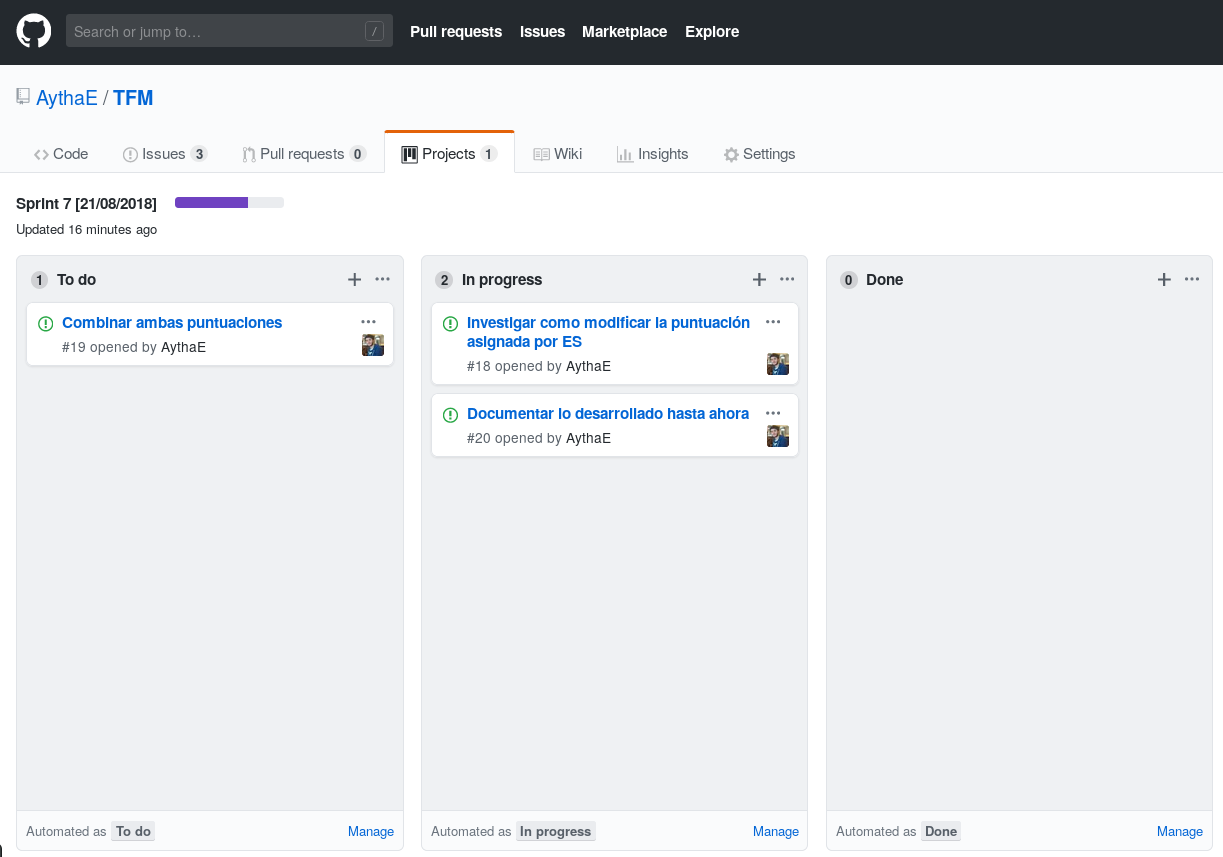
\includegraphics[width=\linewidth]{imagenes/ejemplo_tablero_sprint}
	\caption{Ejemplo de tablero de un \textit{sprint}}
	\label{fig:tableroSprint}
\end{figure}

Además de esto he utilizado un archivo \textit{Markdown} a modo de diario donde ir apuntando cosas interesantes según iban surgiendo, el estado actual de desarrollo o algunas tareas para completar próximamente, dicho fichero se llama \texttt{Diario.md}.

\section{Planificación temporal}

Desde la asignación del \acrshort{TFM}, en diciembre de 2017, me percaté que iba a ser realmente complicado alcanzar la primera convocatoria con la carga de trabajo que suponía el máster. Por lo que decidí tomarlo con calma y llegar a septiembre, pero tras todo finalizar el curso comencé la realización de mis prácticas, lo cual unido a lo extenuado que había acabado el año me impidió alcanzar otra vez el objetivo. 

En Octubre de 2017 comienzo a trabajar, lo cual suponen muchas horas menos al día y me llevo un tiempo adaptarme por lo que no fue hasta Febrero de 2018 cuando me lo empecé a tomar en serio. Teniendo en cuenta mi limitada disponibilidad horaria que apenas me permitía dedicarle 1-2 horas entre diario esbocé una planificación con el objeto de entregar el proyecto en Julio de 2018, dicha planificación inicial se recoge en la siguiente tabla.

\begin{table} [h!]
	\centering
	\begin{tabular}{l c c c}
		\hline
		\textbf{Tarea} & \textbf{Inicio} & \textbf{Fin} & \textbf{Duración}\\
		\hline\hline
		Investigación & 19/02/2018 & 23/04/2018 & 8 semanas \\
		\hline
		Obtención de datos & 23/04/2018 & 07/05/2018 & 2 semanas\\
		\hline
		Procesado de datos & 07/05/2018 & 21/05/2018 & 2 semanas\\
		\hline
		Búsqueda básica & 21/05/2018 & 04/06/2018 & 2 semanas\\
		\hline
		Búsqueda con bibliometría & 04/06/2018 & 02/07/2018 & 4 semanas\\
		\hline
		Refinamiento & 02/07/2018 & 09/07/2018 & 1 semana\\
		\hline
	
	\end{tabular}
	\caption{Planificación inicial de tareas}
\end{table}

Desgraciadamente las vacaciones que he tomado entre medias junto con algunos imprevistos no me permitieron llegar a tiempo aunque ya tenía el proyecto encaminado.

\chapter{Contexto}


\section{Recuperación de información}
La \textbf{\acrfull{RI}} es una disciplina que trata de modelar, diseñar e implementar sistemas capaces de promocionar acceso basado en contenidos. \cite{RIspaBook}

En general un sistema de \acrshort{RI} recibe una petición o consulta  del usuario y debe devolver de entre su conjunto de información las unidades relacionadas con la consulta. 

Estas unidades pueden representar cualquier tipo de elemento: ficheros de texto, imágenes, archivos de audio, etc. De forma genérica se denominan \textbf{documentos} así como al conjunto de información se le denomina \textbf{colección}.



\subsection{Relevancia y similitud}
La \textbf{relevancia} hace referencia a la relación entre la consulta de un usuario y los documentos recuperados. Por ello intuitivamente se entiende que un documento es relevante para una consulta concreta si contribuye a satisfacer la necesidad de información expresada por la misma. Aunque el concepto pueda parecer claro, la relevancia no es para nada absoluta, es una media subjetiva que depende de varios factores como quien la valore o como se haya planteado la consulta inicial.

Respecto a la \textbf{similitud} esta es una medida de semejanza entre documentos o entre documentos y consultas. Otra vez más nos encontramos ante una medida relativa y que se puede medir de diversas maneras: comparación de cadenas de texto, uso de un mismo vocabulario, que dos documentos pertenezcan al mismo autor, que dos documentos tengan múltiples referencias comunes...\cite{ApuntesRI}


\subsection{Las tres dimensiones de la \acrshort{RI}}
Se puede decir que las tres dimensiones principales de la \acrshort{RI} son:\cite{RIspaBook}

\subsubsection{Acceso a la información}
Como puede acceder un usuario a los datos. Existen diversos paradigmas de búsqueda:
\begin{itemize}
	\item \textbf{Clasificación}: cada documento pertenece a clases y estas se pueden usar como jerarquías.
	\item \textbf{Agrupamiento}: documentos se agrupan en conjuntos.
	\item \textbf{Filtrado}: se selecciona un subconjunto de documentos.
	\item \textbf{Recomendación}: los documentos se presentan al usuario basados en su interacción previa con el sistema.
	\item \textbf{Resumen}: fragmentos de documentos utilizados para reducir la información presentada al usuario, muy típico de motores de búsqueda web.
\end{itemize}
\subsubsection{Tipos de información}
Hoy en día vivimos en una marea de información muy heterogénea y creciente lo que hace complicado definir los distintos tipos, por citar los principales actualmente:
\begin{itemize}
	\item \textbf{Documentos textuales} como paginas web o \acrshort{PDF}.
	\item \textbf{Partes de un documento}, capítulos o secciones de este.
	\item \textbf{Búsqueda de información multimedia}: como canciones o vídeos a partir de propiedades perceptibles o incluso de otros elementos multimedia, la búsqueda de imágenes en Google imágenes por ejemplo.
	\item \textbf{Búsqueda de e-mails}: implementado en cualquier cliente de correo web o nativo.
	\item \textbf{Búsqueda geográfica}: por nombre del lugar, sitios cercanos...
\end{itemize}
\subsubsection{Colección}
Guarda relación con los documentos que pueden ser buscados y se pueden clasificar tres tipos en función del tamaño:
\begin{itemize}
	\item \textbf{Personal}: ficheros del dispositivo del usuario.
	\item \textbf{Corporativa}: documentos de una empresa, algo más compleja, supone búsqueda en múltiples ubicaciones conectadas en red.
	\item \textbf{Web}: cualquier documento web, el volumen de datos y la infraestructura es descomunal.
\end{itemize}


\subsection{Componentes de un sistema de \acrshort{RI}}
De manera general un sistema de \acrshort{RI} se compone de los elementos que se observan en la siguiente figura. Ha de contar una interfaz de usuario encargada de recoger las peticiones y mostrar los resultados. Sera necesario interpretar estas consultas para convertirlas en términos que el sistema pueda entender.

\begin{figure}[h]
	\centering
	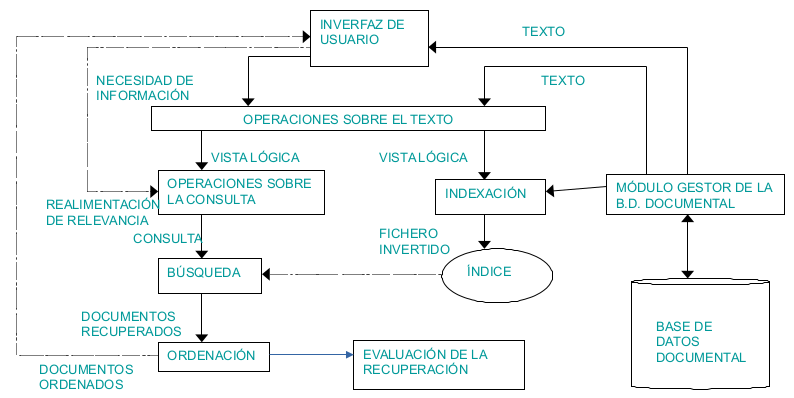
\includegraphics[width=\linewidth]{imagenes/componentes_ri}
	\caption{Componentes de un sistema RI \cite{ApuntesRI}}
	\label{fig:componentes RI}
\end{figure}

Una vez hecho esto el algoritmo de búsqueda encontrara los documentos que sean relevantes para la consulta, tras esto sera necesario puntuar estos documentos recuperados y devolver esta lista puntuada al usuario.

Para realizar este proceso de búsqueda y priorización se servirá del \textbf{índice}, una o varias estructuras de datos que permiten optimizar la búsqueda sobre una colección. En su forma más básica se trata de una estructura que relaciona términos con los documentos en los que aparecen, de modo que si una consulta contiene esos términos se devuelven los documentos que los contienen.

\subsection{Modelos}
\label{subsc:modelos}
Se puede definir un modelo de \acrshort{RI} como una especificación de la forma de representar documentos, consultas y realizar comparaciones entre ambos \cite{ApuntesRI}. El objetivo final es calcular una puntuación para cada documento dada una consulta especifica que determine el grado de relevancia de este, utilizando esa medida se puede llevar a cabo una ordenación o ranking de los documentos. 

Los modelos clásicos a pesar de ser los más básicos sirven como base para crear otros más complejos como alguno de los que se hablará posteriormente. Estos modelos clásicos son:\cite{RIspaBook}

\begin{list}{}{}
	\item  El \textbf{Modelo booleano} basado en teoría de conjuntos y lógica booleana. Se define el conjunto \textit{V} como todas las palabras clave de la colección, \textit{V = \{\(t_1, t_2, ..., t_M\)\}}, así mismo se define el conjunto \textit{D} como el conjunto de todos los documentos de la colección \textit{D = \{\(d_1, d_2, ..., d_n\)\}}. 
	
	Cada documento \(d_i\) se representa por tanto como un conjunto de términos que aparecen en él, este es un subconjunto de \textit{V}. Las consultas en este modelo se representan mediante las operaciones booleanas típicas AND, OR y NOT.
	
	\item El \textbf{Modelo vectorial} modela los documentos y consultas como vectores de términos en un espacio vectorial de dimensión definida por el número de términos de la colección. 
	
	Cada documento es por tanto un vector en dicho espacio vectorial. Usando los conjuntos descritos en el modelo previo se puede definir un documento \(d_i\) como el vector de términos \(\vec{d_i} = (w_{1,i}, w_{2,i}, ..., w_{M,i})\) donde \(w_{i,j}\) representa el peso del término i en el documento j.
	
	Queda por determinar el esquema de pesos y la función de similitud entre vectores.
	
	\item El \textbf{Modelo probabilístico} pretende expresar la relevancia de los documentos utilizando la teoría de probabilidades, por tanto se define \(P(Rel|d, q)\) como la probabilidad de que dado un documento \textit{d} y una consulta \textit{q} el documento sea relevante con cierta probabilidad. 
	
	Simplificando la notación a $P(Rel|d)$ y usando el \gls{Bayes}\glsrefentry{Bayes} podemos transformar el cálculo de esa probabilidad en:
	\begin{equation}
	P(Rel|d) = \frac{P(d|Rel)P(Rel)}{P(d)}
	\end{equation}
	
	
	La función de similitud en el modelo probabilístico se expresa como:
	\begin{equation}
	sim(q,d) = \frac{P(Rel|d)}{P(\overline{Rel}|d)}
	\end{equation}
	Es decir el ratio entre la probabilidad de que un documento sea relevante y no para \textit{q}. 
	
	Aplicando la transformación anterior esta función queda como:
	\begin{equation}
	sim(q,d) = \frac{P(d|Rel)}{P(d|\overline{Rel})}\frac{P(Rel)}{P(\overline{Rel})} \approx \frac{P(d|Rel)}{P(d|\overline{Rel})}
	\end{equation}
	Donde $\frac{P(Rel)}{P(\overline{Rel})}$ se conoce como característica independiente de consulta\label{modelProb} al suponer la relación entre las probabilidades de escoger un documento al azar y que este sea relevante o irrelevante, se suele eliminar como simplificación. 
	
	Por otro lado $\frac{P(d|Rel)}{P(d|\overline{Rel})}$ supone la relación entre la probabilidad sabiendo que un documento es relevante este sea \textit{d} y su inversa. Estas probabilidades resultan más fáciles de calcular y son las utilizadas en estos modelos.
	
	
\end{list}
\subsection{Contexto histórico}
La historia de la \acrshort{RI} comienza antes de la era digital. Como ejemplo las tablas de contenidos e índices de un libro forman un sistema de \acrshort{RI} a pequeña escala, los índices relacionan \gls{termIndex} con su ubicación en el documento de forma similar a un glosario de términos, ver \glsrefentry{termIndex} .

Esto es lo que se conoce como búsqueda \textbf{pre-coordinada} donde los términos de búsqueda o consultas están definidas de antemano, esto hace que se pueda organizar muy bien la información (como se hace en una biblioteca por ejemplo), pero requiere que el usuario conozca estos términos y no supone un método muy escalable teniendo en cuenta el volumen de información manejado en sistemas actuales. Por ello surgió la \textbf{post-coordinación} en la década de 1950 que se basa en definir las consultas en el momento de la búsqueda, dándole libertad al usuario.

A este último enfoque pertenecen la mayoría de los sistemas actuales, los cuales recibieron un enorme impulso con el desarrollo de la web iniciado en 1989 por Tim Berners-Lee en el CERN. Los primeros buscadores web de la forma que los conocemos hoy surgieron entorno a 1994, sistemas como Lycos o Altavista. 

La búsqueda de documentos en la web siempre ha resultado un reto debido a su naturaleza heterogénea, la propuesta de unos jóvenes estudiantes de la universidad de Stanford en 1998 supuso una revolución y asentó lo que hoy conocemos como buscador. Esa propuesta fue el algoritmo \textit{PageRank}\cite{PageRankPaper} y esos chicos eran Larry Page, Sergey Brin, Rajeev Motwani y Terry Winograd; los dos primeros fundaron poco después una empresa llamada Google, que a día de hoy es el buscador más utilizado. \cite{searchEngineShare}

Hoy en día existe una dependencia casi absoluta por los motores de búsqueda para navegar por internet, lo que hace de este un tema tan crucial en el que aún se sigue trabajando, con retos aún por delante como el enorme tamaño que ha alcanzado la web, la heterogeneidad de contenido con cada vez más contenidos multimedia o el acceso desde cualquier tipo de dispositivo y desde cualquier lugar. 

\section{Bibliometría}
\label{sc:bibliometria}
\subsection{Definición}
La \textbf{bibliometría} se puede definir como el análisis estadístico de publicaciones escritas. Sus métodos se suelen utilizar para ofrecer un análisis cuantitativo de la literatura académica \cite{de2009bibliometrics}. Se relaciona mucho con la \textbf{cienciometría} que se puede entender como el estudio cuantitativo de la ciencia de forma general \cite{DBLP:journals/corr/abs-1208-4566}. 

Específicamente para este trabajo resulta destacable el enfoque de poder medir la importancia de trabajos científicos de forma cuantitativa y como esto se puede utilizar para mejorar los resultados de un sistema \acrshort{RI}. Yendo al uso más particular que se llevara a cabo durante el desarrollo de este trabajo ambas disciplinas proponen una serie de medidas particulares, algunas de las cuales comentaré en el siguiente apartado.

\subsection{Medidas}
\subsubsection{Número de citas} \label{numero_citas}
Esta es una de las métricas más directas y sencillas, se basa la premisa de que un documento científico es más relevante si cuenta con mayor número de citas. Actualmente se encuentra disponible en casi cualquier plataforma bibliográfica como Google Schoolar, Scopus o Web of Science. 

Sobre esta métrica básica se han construido muchas posteriormente como el impacto de citas (media de citas por documento), el impacto de citas ponderado por el campo (la anterior pero ponderado por materia, tipo de publicación y año), \textit{Highly cited papers} (documentos en el top 1 \% de citas ponderado por campo y año)\cite{BibliometricWhitePaper}, \textit{CiteScore} (media de citas anuales para todos los documentos de una revista concreta durante los últimos 3 años), \textit{SCImago Journal Rank} (medida que pondera el número de citas de una revista científica con el prestigio de las que la citan) o \textit{SNIP} (normalización del número de citas de un paper por su impacto en la materia) \cite{bibliometric_measures}.
\subsubsection{Análisis de co-citación}

Medida de similaridad que establece que dos documentos serán semejantes si aparecen citados conjuntamente con frecuencia por otros documentos. Sobre esta premisa se puede considerar un índice de co-citación que es simplemente el número de citas co-citaciones de 2 documentos. 

También existen métricas más complejas como el análisis de co-citación por proximidad que incorpora a la idea previa el hecho de si dos citas aparecen en la misma sección del texto estas estarán más relacionadas que si una aparece en la introducción y otra en las conclusiones por ejemplo. \cite{Gipp09a}

\subsubsection{Índice h}
Este índice se puede aplicar a un autor científico, el índice h de un autor es x si este tiene x artículos con al menos x citas \cite{BibliometricWhitePaper}. Se utiliza ampliamente para medir la productividad de un investigador.

Tiene diversas variantes como el índice g (índice h para el número de citas medio), índice m (corrección del índice h con el tiempo) o el índice Py (número medio de publicaciones por año).

\subsubsection{Acoplamiento bibliográfico}

Muy relacionado con el análisis de co-citación, el acoplamiento bibliográfico o \textit{bibliographic coupling} basa su concepto de similaridad en que 2 documentos serán semejantes si comparen citas.

En base a esta idea se puede crear un métrica simple que sea el número de referencias comunes entre dos documentos, o medidas más complejas como el acoplamiento bibliográfico entre autores que supone el acoplamiento entre el conjunto de citas de todos los trabajos de un autor con otro \cite{authorBiblioCoupling}.


\subsubsection{Altmetrics}  \label{altmetrics}
Conjunto de medidas relativas al mundo \textit{online}, veces que un documento ha sido descargado, compartido, mencionado en la redes sociales, blogs, wikipedia... \cite{almetrics}

Existen diversas compañías que ofrecen productos sobre estás métricas siendo una de las principales \href{https://www.altmetric.com/}{Altmetric}. Entre sus productos destaca el "donut" que se puede apreciar en la siguiente imagen. Este corresponde con una medalla que puede colocar en la página de un articulo y permite de un vistazo la atención que esta generando este trabajo. También incluye información en detalle de donde se esta hablando del mismo incluyendo comentarios en redes sociales.

\begin{figure}[h]
	
	\centering
	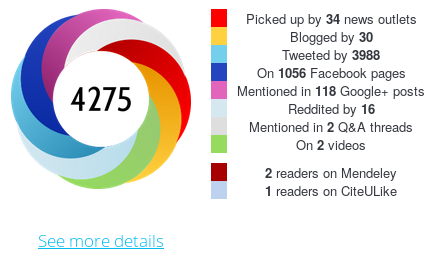
\includegraphics[width=0.7\linewidth]{imagenes/altmetrics_donough}
	\caption{Donut de Altmetric}
	\label{fig:altmetricsdonough}
\end{figure}


\subsection{Limitaciones}
Estas medidas ayudar dar una idea la importancia de un documento o de la productividad de un autor, pero no deben de ser tomadas como únicos criterios ya que presentan sus limitaciones.

Respecto a las medidas basadas en número de citas son muy dependientes de las fuentes de las que tomen datos así como su cobertura, por otro lado que un articulo sea muy citado no quiere decir que este sea muy influyente, se puede citar un trabajo para criticarlo. También hay que tener en cuenta las <<auto citas>> citas de un autor a otros trabajos suyos que pueden distorsionar estas medidas \cite{BibliometricWhitePaper}.

No se puede comparar categóricamente dos trabajos o autores de cualquier disciplina usándolas, ya que en distintos campos se cita de manera distinta. 

En las medidas que dependan de citaciones (prácticamente todas) hay que considerar un factor temporal, para que un trabajo adquiera relevancia es necesario cierto tiempo, por ello se recomienda dejar fuera las publicaciones recientes (de los últimos tres años)\cite{BibliometricWhitePaper}.
% Interesante hacer un apartado de plataformas bibliográficas ???


\section{Combinando ambas disciplinas}

En los últimos años han surgido diversos trabajos que proponen combinar ambas disciplinas, utilizar la bibliometría para mejorar la recuperación de información. Esto no se puede aplicar de manera genérica y directa a cualquier sistema de \acrshort{RI} ya que la bibliometría esta muy centrada en el mundo de la académico y de la investigación, sin embargo con algunas adaptaciones las ideas de la bibliometría se encuentran muy presentes en los sistemas de \acrshort{RI}, por ejemplo el algoritmo PageRank hace una analogía entre páginas web con artículos científicos así como hiperenlaces con citas en los mismos \cite{PageRankPaper}. 

\subsection{Sistemas de \acrshort{RI} actuales con medidas bibliométricas}
\label{subsec:sistemasRI}
Donde resulta obvio que esta combinación puede ser beneficiosa es los sistemas \acrshort{RI} especializados en literatura académica siendo los más importantes:

\begin{itemize}
	\item \href{https://scholar.google.es/}{Google Scholar}: buscador gratuito especializado en literatura científica, contiene algunas medidas bibliométricas con el número de citas o el índice-h de un autor. Sin embargo ha sido muy criticado por intentar incluir el mayor número de artículos posibles sin importar la calidad de los mismos \cite{googleScholarJunk} o dar demasiada importancia al número de citas lo que hace que sea complicado descubrir nuevos trabajos que no son muy conocidos \cite{Beel09}.
	
	\item \href{http://wos.fecyt.es/}{\acrfull{WoS}}: Sistema de RI por subscripción más utilizado, habitualmente las instituciones académicas lo tienen contratado, como es el caso de la \acrlong{UGR} a través de la \acrfull{FECYT}. Agrupa múltiples bases de datos de diversas índoles llegando a tener más de 100 millones de documentos \cite{WoS_Facts}. Fue uno de los primeros sistemas en aparecer y actualmente pertenece a Clarivate Analytics. A diferencia de Google Scholar los contenidos son revisados por expertos antes de ser incluidos \cite{WoS_Facts}. 
	
	\item \href{https://www.scopus.com/}{Scopus}: Similar a \acrshort{WoS}, en este caso pertenece a la editorial Elsevier. También se puede usar desde la \acrshort{UGR} gracias a la \acrshort{FECYT}. Este sistema es más reciente, cuenta con unos 70 millones de documentos \cite{scopus} y también tiene un proceso de revisión de contenido. Dispone de algunas otras medidas de bibliometría además del número de citas o índice-h, como los otros sistemas descritos, cuenta con las medidas \textit{CiteScore}, \textit{SCImago Journal Rank} y \textit{SNIP} (ver \ref{numero_citas} para más información). 
\end{itemize}

\subsection{Trabajos relacionados}
\label{subsc:trabajosRelacionados}
Desde un punto de vista académico resultan especialmente interesantes los trabajos de los talleres \acrfull{BIR}. Estos congresos se celebran anualmente desde 2014 y tienen como objetivo "\textit{hacer consciente a la comunidad de \acrshort{RI} de sus posibles vínculos con la bibliometría}" \cite{DBLP:conf/ecir/X14}. Voy a destacar algunos de ellos a continuación.

% Re ordenar resultados usando alguna medida, uso de altmetrics
Ante el creciente volumen de trabajos científicos se hace complicado para investigador mantenerse al día en su propio campo porque resulta imposible leer todos los trabajos, por ello se suele utilizar algún \gls{recomenderSystem} \glsrefentry{recomenderSystem}. Pero los sistemas existentes no contemplan bien el uso de medidas bibliométricas para distinguir los trabajos relevantes, por ello en \cite{DBLP:conf/ecir/SiebertDF17} se propone reordenar la salida del sistema de recomendación \href{mr-dlib.org}{\acrshort{Mr.DLib}} utilizando como criterio varias medidas derivadas del número de lectores de un artículo, un tipo de \textit{altmetric} (ver \ref{altmetrics}). Las conclusiones de este trabajo demuestran que se encuentra una mejora utilizando las medidas de cienciometría solas o en combinación con el ordenamiento normal basado en texto que usando solo el ordenamiento del sistema \acrshort{RI}, siendo la métrica que mejor resultado obtuvo el número absoluto de lecturas sin normalización. Esta mejora no es muy significativa como cabría esperar, los autores achacan esto a la falta de cobertura de datos bibliométricos en la colección.

% Modelo más clásico, priores con medidas biblio
Otro enfoque interesante es el de \cite{DBLP:conf/ecir/ZhaoH14}, donde se propone utilizar medidas bibliométricas como variables independientes de consulta o \textit{static features}, ver el modelo probabilístico \ref{modelProb}. Estás características se conocen como priores en el modelo probabilístico de lenguaje utilizado y modifican la probabilidad de que un documento sea relevante para una consulta dada, multiplicando dicha probabilidad por un factor. Para realizar su estudio han utilizado la colección bibliográfica de prueba iSearch, que desgraciadamente parece no estar disponible ya. De esta colección seleccionaron el subconjunto de artículos con al menos alguna cita dentro de la colección (para poder llevar acabo un análisis de co-citación). 

Como priores han seleccionado la proporción de citas dentro del subconjunto de documentos entre el número total de estas, el \textit{PageRank} calculado en el subconjunto y el clustering de co-citación \footnote{creando un grafo no dirigido con peso de citas donde los nodos son documentos y las aristas citas, sobre el que se aplica un algoritmo de clustering y se calculan los priores del cluster mediante validación cruzada de 5 iteraciones}, siendo todas las variantes también suavizadas con una versión logarítmica. Aunque el concepto es interesante y el método exhaustivo los resultados obtenidos no son significativos, se achaca esto al bajo tamaño de la colección de prueba, con 863 documentos.

% Otro modelo clásico, tf*idf sobre trabajos en lugar de términos usando co-citación como métrica
Siguiendo un modelo vectorial pero aplicando una variación del conocido esquema de pesos \textit{tf*idf} se encuentra \cite{DBLP:conf/ecir/White16}. En el esquema de ponderación para los términos original \textit{tf} representa la frecuencia de un término en el documento e \textit{idf} el número de documentos donde aparece el término a la inversa. Con ello se consigue dar mayor importancia a los términos que aparezcan menor número de veces ya que serán más discriminantes e importantes para una búsqueda.

El modelo propuesto en este paper apuesta por buscar documentos en función de otros, es decir los términos de consulta son otros documentos de la colección, los cuales se conocen como semillas. Para la ponderación de peso en cada documento ahora \textit{tf} es el número de documentos co-citados con el documento semilla e \textit{idf} la inversa del número total de citas entre documentos de la colección. Por último cita algunos ejemplos sobre colecciones de prueba y discute el modelo planteado sin llegar a evaluarlo realmente. De este, se dice que sería especialmente útil para usuarios con conocimiento previo del dominio, por ejemplo para llevar acabo una investigación bibliográfica sobre algún autor.

Basado parcialmente en el trabajo previo, el siguiente artículo \cite{DBLP:conf/ecir/SarolLS18} propone la creación de un \gls{framework} \glsrefentry{framework} para llevar a cabo una investigación bibliográfica siguiendo un enfoque híbrido combinando información textual y de citación. A partir de la selección de algunos documentos semilla, el sistema crea el espacio de citaciones \footnote{Documentos citados por las semillas, aquellos que las citan a ellas y documentos con relación de co-citación con estas}, sobre el cual se filtra poniendo condiciones, el resultado de este filtrado se refina buscando términos y frases comunes con las semillas en el resumen de los documentos. 

Utilizan su sistema para comparar con diversos trabajos de revisión bibliográfica realizados manualmente con el objetivo de lograr obtener el mismo conjunto final de documentos relevantes revisando menos trabajos con lo que se ahorraría un tiempo significativo. Sus resultados resultan prometedores, usando todas las combinaciones de 3 documentos semilla entre los seleccionados finalmente por cada revisión logran recuperar todos los documentos finales disponibles en Scopus (plataforma en la que realizan el estudio) reduciendo el número de documentos totales recuperados para esa revisión en hasta el 80 \% dependiendo de la revisión concreta.







%

%

%
%\input{capitulos/04_Analisis}
%
\chapter{Diseño}


\section{Fuentes de datos}
Al ser este un sistema \acrshort{RI} el diseño ha de girar en torno a los datos, por ello comencé explorando diversas alternativas para utilizar como fuente de datos. 

Como punto inicial para la extracción de los datos de los autores de la \acrshort{ETSIIT} partí del Ranking UGRinvestiga \cite{Ranking_UGRInvestiga}. En este se lista a todos los autores de la escuela junto con sus citas e índice h total y los últimos 5 años.

Sin embargo no hay modo de obtener datos de los artículos concretos por lo que barajé múltiples bases de datos bibliográficas, además de las ya comentadas en la sección \nameref{subsec:sistemasRI} también exploré \href{https://www.researchgate.net/}{Research Gate}.

Los resultados de mi análisis fueron los siguientes: 
\label{ls:dataSourceAnalisis}
\begin{itemize}
	
	\item Google Scholar y Research Gate parecen tener bastantes datos en comparación a otras opciones, sin embargo no ofrecen una \acrshort{API} por lo que la extracción de datos solo se podría llevar a cabo mediante \textit{\gls{webscraping}} \glsrefentry{webscraping}. Esto no es un proceso sencillo, ya que muchas de estas web contienen mecanismos de detección de bots como los CAPTCHAs \cite{scrapping_GS} y además es un método muy sensible al cambio: en caso de que produzca alguna modificación en la web en cuestión es probable que toque reescribir el método de extracción de datos.
	\item \acrshort{WoS} y Scopus sí disponen de una \acrshort{API}, tras realizar algunas pruebas y leer opiniones sobre ambas me decanté por utilizar Scopus como fuente de datos ya que su \acrshort{API} me resultó más cómoda de utilizar y encontré datos fácilmente de algunos autores de la \acrshort{ETSIIT} (cosa que me costó bastante más en \acrshort{WoS}).
\end{itemize}

\section{Modelo de datos}

Siguiendo el modelo de Scopus decidí separar la búsqueda de autores y la de artículos como apunté en los objetivos.

Por tanto mi modelo de datos está constituido por 2 entidades distintas pero relacionadas: Autores (\textit{Author}) y Artículos (\textit{Abstract}). 

En las siguientes secciones se describen brevemente ambas entidades.


\subsection{\textit{Author}}
\label{subsc:author}
Esta entidad es resultado de la combinación de la información disponible en el Ranking UGRinvestiga \cite{Ranking_UGRInvestiga} y en Scopus, por eso podemos ver en el siguiente diagrama con el prefijo \texttt{ugr} las medidas de dicho ranking y con el de \texttt{scopus} los de la plataforma homónima. 

Respecto a los atributos que finalizan en \texttt{5} estos hacen referencia a los valores de dichas medidas de los últimos cinco años.

\begin{figure}[ht]
	
	\centering
	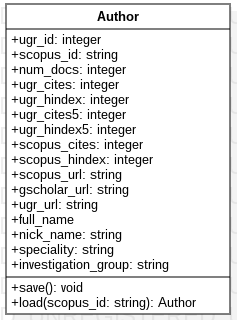
\includegraphics[width=0.5\linewidth]{imagenes/Author}
	\caption{Clase \textit{Author}}
\end{figure}

\newpage

\subsection{\textit{Abstract}}
\label{subsc:abstract}
La entidad \textit{Abstract} corresponde casi directamente con los datos obtenidos a través de la \acrshort{API} de Scopus, a excepción de:
\begin{itemize}
	\item Las referencias han sido limitadas a citas internas, es decir entre los artículos que están disponibles en la colección, con la idea de usar esta información en el proceso de búsqueda.
	\item Los autores, que únicamente aparecían listados con su \texttt{scopus\_id}, han sido enriquecidos con el nombre de los mismos así como el \texttt{ugr\_id} en caso de estar disponible este último (este identificador estará disponible si el autor es alguno de los que forman parte de la colección de autores).
\end{itemize}

\begin{figure}[h]
	
	\centering
	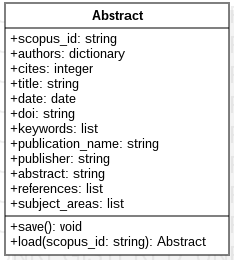
\includegraphics[width=0.5\linewidth]{imagenes/Abstract}
	\caption{Clase \textit{Abstract}}
\end{figure}

\newpage

\section{Arquitectura inicial del sistema}
\label{sc:arq_inicial}
La arquitectura del sistema planteado se basará en el modelo cliente/servidor con tres nodos:
\begin{itemize}
	\item \textbf{Servidor de \acrlong{BD}}: El cual almacenara la información correspondientes a autores y artículos como se ha modelado en el apartado previo.
	\item \textbf{Servidor de \acrshort{RI}}: Donde se llevará a cabo la búsqueda en sí, se servirá del servidor de \acrshort{BD} como almacenamiento de datos y atenderá las peticiones de búsqueda.
	\item \textbf{Cliente}: Parte del sistema que será visible para el usuario y que se encargará de recoger las peticiones de búsqueda, enviarlas al servidor de \acrshort{RI} y presentar los resultados devueltos por el mismo
\end{itemize}

\begin{figure}[ht]
	
	\centering
	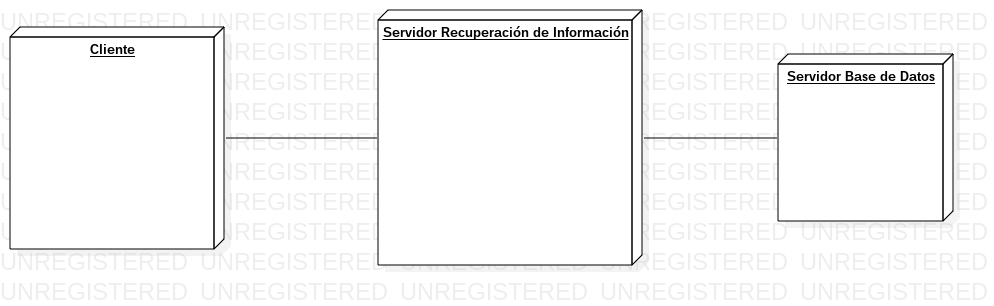
\includegraphics[width=\linewidth]{imagenes/initial_architecture}
	\caption{Diagrama de arquitectura inicial del sistema}

\end{figure}

\chapter{Técnicas y herramientas [Aún en progreso]}
\label{ch:herramientas}

Comentar en más detalle todas las herramientas utilizadas con enlaces de cada una.

\begin{itemize}
	\item \textbf{Debian}: \acrfull{SO}.
	\item \textbf{Python}: Lenguaje de programación usado en las primeras fases del proyecto y en servidor \gls{backend} \glsrefentry{backend}.
	\item \textbf{JavaScript}: Lenguaje de programación interpretado en el que se ha escrito el \gls{frontend} \glsrefentry{frontend}.
	\item \textbf{Elasticsearch}: Servidor de búsqueda.
	\item \textbf{MongoDB}: Base de datos NoSQL.
	\item \textbf{React}:  \Gls{framework} para el desarrollo de interfaces de usuario.
	\item \textbf{Searchkit}: \Gls{framework} que incluye un conjunto de componentes React para la comunicación con Elasticsearch.
	\item \textbf{TeXstudio}: Entorno integrado de escritura en \LaTeX{} utilizado para generación de la documentación.
	\item \textbf{Docker}: Software de virtualización para basado en contenedores. Permite gestionar de forma simple la gestión y despliegue de una infraestructura software.
	\item \textbf{Visual Studio Code}: Editor de código creado por Microsoft utilizado para toda la programación del proyecto.
	\item Git
	\item GitHub
	\item Pandas
	\item PyMongo
	\item scopus-api
	\item Beautiful Soup
	\item Matplotlib
	\item MaterialUI
	\item elasticsearch-py
	\item Star UML
	\item Cerebro
	\item Flask
	\item Gimp
	\item Nginx
	\item uWSGI
\end{itemize}

\chapter{Desarrollo}
En este capítulo se detallara el proceso de desarrollo seguido dividido en \textit{sprints} como ya se ha comentado en la sección \nameref{sc:metodologia}.


\section{\textit{Sprint} 1}
Este primer \textit{sprint} tiene como objetivo general la investigación básica sobre la \acrshort{RI}. Sus objetivos concretos son: 

\begin{itemize}
	\item Leer el libro \acrlong{RI}: un enfoque práctico y multidisplinar \cite{RIspaBook}.
	\item Buscar los talleres \acrshort{BIR} centrándose en sus editoriales para realizar un listado priorizado por interés de los diversos artículos.
\end{itemize}

Siguiendo la recomendación de mi tutor (co-autor del libro) me centré en los capítulos \textit{"1 Introducción a la recuperación de información"}, \textit{"2 Indexación de documentos y procesado de consultas"}, \textit{"3 Modelos de recuperación de información clásicos"} y \textit{"10 Técnicas de modificación de la consulta"}. 

Esta lectura me hizo adquirir unas bases más teóricas a lo que ya había estudiado en la asignatura del máster \acrlong{GIW} donde obtuvimos una nociones básicas de lo que supone la \acrshort{RI} y sus vertientes realizando alguna práctica.

Los artículos de los talleres \acrlong{BIR} que encontré más destacados están detallados en el apartado \nameref{subsc:trabajosRelacionados} de la Introducción. Dichos trabajos se encuentran disponibles gratuitamente en \url{http://ceur-ws.org/} bajo el amparo de la Universidad Técnica de Aquisgrán (\textit{RWTH Aachen University}) en Alemania.

Cada una de las ediciones de estos talleres se encuentra estructurada dividida en diversos trabajos. Por un lado un editorial que resume la edición y todos los trabajos aceptados en la conferencia así como los trabajos individuales, alguna \textit{keynote} o presentación y algunas demostraciones. 

En este \textit{sprint} me dediqué a leer dichos editoriales clasificando por aparente interés los artículos de cada \acrshort{BIR} generando una lista priorizada utilizada como orden en el que estudiar los trabajos. En la siguiente imagen se puede apreciar el aspecto de dicha lista generada en \textit{Markdown}.

\begin{figure}[ht]
	
	\centering
	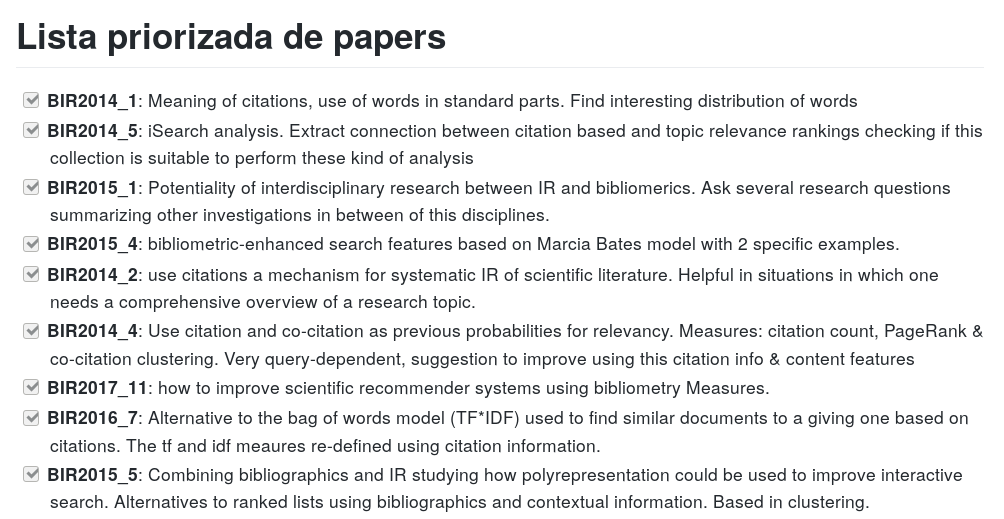
\includegraphics[width=\linewidth]{imagenes/lista_priorizada}
	\caption{Fragmento de la lista priorizada creada}
\end{figure}

\section{\textit{Sprint} 2}
Para el segundo \textit{sprint} plantee el indagar en la \acrshort{RI} e ir introduciendo la bibliometría. Sus objetivos concretos son: 

\begin{itemize}
	\item Leer los primeros 17 papers de los \acrshort{BIR} resumiendo y extrayendo ideas interesantes para el proyecto.
	\item Buscar información sobre medidas bibliométricas (Citas, índice h combinado...)
\end{itemize}

A partir de la lista priorizada fui leyendo los primeros artículos, el orden de esta lista lo fui alterando ya que con frecuencia al indagar en el trabajo este perdía o incrementaba su interés. Con el objetivo de poder aprovechar más estas lecturas fui creando una especie de resúmenes en los que anotaba los puntos más importantes que se trataban en el artículo, otros artículos relacionados de los que se hablaba o los resultados obtenidos con su trabajo. En la siguiente imagen se puede apreciar uno de estos "resúmenes":

\begin{figure}[h!]
	
	\centering
	
\includegraphics[width=\linewidth]{imagenes/paper_sumary}
	\caption{Ejemplo de resumen de uno de los papers}
\end{figure}

En este momento me empecé a introducir en el mundo de las medidas bibliométricas, ya que no tenía conocimiento previo alguno de que existiera esta disciplina siquiera, mediante la lectura de artículos iba descubriendo distintas medidas así como sus posibles aplicaciones a la \acrshort{RI} cuyo resultado final se encuentra sintetizado en la sección \nameref{sc:bibliometria} de la Introducción.

\section{\textit{Sprint} 3}
Ya en este punto decidí que estaba listo para ir documentando todo lo que había aprendido por ello en este \textit{sprint} me puse como objetivo escribir la introducción de este \acrshort{TFM}. Los objetivos concretos son:
\begin{itemize}
	\item Escribir la introducción del \acrshort{TFM}.
	\item Pensar un enfoque para el proyecto a desarrollar decidiendo que clase de sistema se desarrollaría.
	\item Continuar leyendo algunos artículos más de los \acrshort{BIR}.
\end{itemize}

Para asimilar y reflexionar sobre todo lo que había leído me puse a escribir la introducción de este trabajo ya que ello me ayudaría a pensar un enfoque correcto. También quería poder mostrar algo a mi tutor para obtener algo de \textit{feedback} por su parte.

Continué leyendo algunos trabajos más con lo que dí por concluida mi proceso de investigación. Uno de esos últimos trabajos fue \cite{DBLP:conf/ecir/SarolLS18} el cual me gustó especialmente ya que pasaban de un modelo teórico a algo más práctico, accediendo a la \acrshort{API} de Scopus e incluyendo ejemplos de su implementación en un repositorio de \textit{GitHub} lo que me llevo a plantear mi modelo híbrido combinando el sistema habitual de un sistema \acrshort{RI} con reordenamiento de resultados \textit{a priori} usando medidas bibliométricas y un ordenamiento \textit{a posteriori} utilizando un grafo de citación entre los documentos.

Desgraciadamente estos enfoques dependen ampliamente de la cobertura de medidas bibliométricas disponibles, por ejemplo me hubiera encantado poder probar una reordenación previa utilizando alguna \textit{altmetric} como el número de lecturas o descargas de un artículo, pero la plataforma que he utilizado para extraer los artículos no dispone de dichas medidas.

Como parte adicional de este sprint también estuve haciendo alguna pruebas con \glspl{framework} de búsqueda. Como he dicho previamente ya había utilizado \textit{Lucene} como parte de las prácticas de la asignatura \acrshort{GIW}, pero me pareció demasiado bajo nivel así que me centré en investigar otras alternativas. Encontré que las principales, que casualmente utilizaban por debajo \textit{Lucene}, eran \textit{\textbf{Solr}} y \textit{\textbf{\acrlong{ES}}}.

Buscando alguna comparativa \cite{ES_Solr} y comentarios de usuarios en plataformas tan reputadas como \textit{StackOverflow} \cite{ES_Solr_SO} parecía que se recomendaba \acrshort{ES} por ser más sencillo de usar por lo que realicé un breve tutorial \cite{ES_tutorial} que me gustó bastante ya que resulta realmente simple de usar y basta únicamente con realizar consultas sobre una \acrshort{API} \acrshort{REST} por lo que basta con hacer peticiones \acrshort{HTTP} con algún cliente simple como \texttt{curl}. Todo esto hizo que me decidiera por este servidor de búsqueda.


\section{\textit{Sprint} 4}

\section{\textit{Sprint} 5}

\section{\textit{Sprint} 6}

\section{\textit{Sprint} 7}

\section{\textit{Sprint} 8}
%
%\input{capitulos/06_Implementacion}
%
%\input{capitulos/07_Pruebas}
%
\chapter{Conclusiones y Trabajos Futuros}

\section{Relación del \acrshort{TFM} con lo aprendido en el Máster}

GIW

SSBW

CC


\section{Conclusiones}

Proyecto interesante

Curiosidad planteada en la motivacion satisfecha

No tiempo suficiente para llevar a cabo todo lo planteado. Objetivo de  Evaluación no cumplido

\section{Trabajos futuros}
Relevance feedback

Redes de citación

Intentar obtener Altmetrics de otras fuentes

\textbf{Evaluar la mejora producida al aplicar medidas bibliométricas al sistema}: como colección de datos del sistema \acrshort{RI} a desarrollar se ha decidido utilizar el conjunto de todos los trabajos de autores de la \myFaculty lo que favorece que esta evaluación se pueda llevar a cabo, aunque esta no es una tarea sencilla. La evaluación de sistemas \acrshort{RI} se suele llevar a cabo mediante colecciones de prueba donde existe un conjunto de documentos, un conjunto de consultas y un conjunto de resultados que deberían de retornar las mismas  \cite{RI_Evaluation}. Al crear un sistema nuevo con una colección de documentos no utilizada no podemos comparar los resultados obtenidos con los que se esperarían, este problema se debe a la relatividad del concepto de relevancia. Por ello las colecciones de pruebas suelen incluir valoraciones de relevancia de expertos en la materia.
%
%%\chapter{Conclusiones y Trabajos Futuros}
%
%
%\nocite{*}
\bibliographystyle{ieeetr}
\bibliography{bibliografia/bibliografia} \addcontentsline{toc}{chapter}{Bibliografía}

\appendix
\clearpage
\addappheadtotoc
\appendixpage

%%\input{apendices/paper/paper}



\printnoidxglossary[sort=use]
%\addcontentsline{toc}{chapter}{Glosario}

\printnoidxglossary[type=\acronymtype, title=Lista de Acrónimos]
%\addcontentsline{toc}{chapter}{Lista de Acrónimos}
\chapter{Manual técnico de uso}

\section{Descripción de la arquitectura}
El sistema desarrollado a lo largo de este proyecto se ha servido de \textit{Docker} como forma de gestionar la infraestructura de los diversos nodos que lo conforman. La arquitectura final del sistema como se recoge en la figura \ref{fig:finalArchitecture} se constituye de 4 nodos o contenedores \textit{Docker} concretamente.

\begin{itemize}
	\item \textit{\textbf{app}}: contenedor que contiene una imagen con un servidor \textit{Nginx} encargado de servir el \gls{frontend} \textit{React} y el cual se comunica con servidor de aplicación \textit{uWSGI} mediante un \textit{socket UNIX}. Dicho servidor de aplicación sirve la aplicación \textit{Flask} que constituye el \gls{backend} del sistema.
	\item \textit{\textbf{elasticsearch}}: contenedor en el cual se encuentra alojada una imagen de \acrlong{ES} en su versión \textit{Open Source} siguiendo las instrucciones oficiales \cite{ES_docker}.
	\item \textit{\textbf{mongodb}}: contenedor con la imagen de \textit{MongoDB} utilizada
	\item \textit{\textbf{cerebro}}: contenedor con el servicio de monitorización de \acrshort{ES} \textit{Cerebro}. Este contenedor no es necesario para el funcionamiento del sistema pero ha resultado muy útil durante el desarrollo para gestionar el contenedor de \acrshort{ES}
\end{itemize}

\section{\texttt{docker-compose.yml}}
En el siguiente listing se observa la configuración del fichero \texttt{docker-compose.yml} que determina la infraestructura descrita arriba.

\lstinputlisting[language=yaml, caption=Fichero \texttt{docker-compose.yml} de la aplicación]{code/docker-compose.yml}

\section{Instalación}
\subsection{Docker y Docker Compose}
Para poder desplegar la aplicación por tanto lo primero sera instalar \textit{Docker} y \textit{Docker Compose}. Para instalar \textit{Docker} se ha utilizado su versión \textit{Community Edition (CE)} por ello ver las instrucciones de instalación para el sistema en el que se desee instalar \cite{dockerInstall}. Respecto a \textit{Docker Compose} recomiendo instalar la versión nativa para el sistema de destino en lugar de utilizar las opciones alternativas de instalación, ver la documentación oficial en \cite{dockerComposeInstall}.

\newpage

\subsection{Descripción del repositorio}
Una vez instalado esto sera necesario \textit{clonar} el repositorio de \textit{GitHub}, que recuerdo era \url{https://github.com/AythaE/TFM}, cuya estructura se observa a continuación. Para disponer de los datos de \textit{MongoDB} y \acrlong{ES} será necesario descomprimir el fichero \texttt{data.7z}. Esto creara una carpeta \texttt{data}.

\dirtree{%
.1 TFM.
.2 data/.
.3 es\_data/.
.3 mongodb\_data/.
.2 config/.
.3 elasticsearch.yml.
.2 src/.
.3 backend/\DTcomment{Código \gls{backend} y fichero \texttt{requirements.txt} con las dependencias de \textit{Python}}.
.3 frontend/\DTcomment{Código \gls{frontend} y fichero \texttt{package.json} con las dependencias de \textit{JS}}.
.3 Exploring/.
.4 elasticsearch/\DTcomment{Código de indexación en \acrshort{ES}}.
.4 Exploratory\_analysis/\DTcomment{Ficheros y gráficos generados en el análisis de datos}.
.4 investigadores/\DTcomment{Código extracción de datos del ranking UGRinvestiga}.
.4 scopus/\DTcomment{Código extracción de datos de Scopus}.
.3 Dockerfile\DTcomment{Fichero que dertermina la construcción del contenedor \textit{\textbf{app}}}.
.2 docker-compose.yml.
}

\section{Despliegue}
Con todo esto ya estamos listos para desplegar la aplicación. Para ello basta con ejecutar el siguiente comando desde el directorio \texttt{TFM}:

\begin{lstlisting}[style=Consola, caption=Comando para desplegar el sistema]
$ docker-compose -f "docker-compose.yml" up --build
\end{lstlisting}

Una vez finalice la construcción del contenedor \textbf{\textit{app}} se mostrarán unos mensajes indicando que todos los contenedores han arrancado correctamente, tras esto podremos acceder a \url{http://localhost} donde se encontrará desplegada la aplicación.

En caso de algún problema en el despliegue esto seguramente se deba a los puertos disponibles, el sistema utiliza los puertos 80 (acceso \acrshort{HTTP} \gls{frontend}), 27017 (\textit{MongoDB}), 9000 (\textit{Cerebro}), 9200 y 9300 (\acrlong{ES}). Por lo que si alguno de esos puertos se encuentra en uso el despliegue fallará. Dicho mapeo de puertos se puede cambiar fácilmente modificando los \texttt{ports} en el fichero \texttt{docker-compose.yml}.


Para parar la aplicación basta con aplicar un \texttt{Ctrl\^\ C} sobre la consola donde se esté ejecutando el comando de despliegue.




\chapter*{}
\thispagestyle{empty}

\end{document}
